\lab{Data Visualization}{Data Visualization} 
\objective{Use data visualizations to explore data and communicate it to others.}
\label{lab:DataVis}

\noindent\emph{The purpose of visualization is insight, not pictures.} \small{---Card, Mackinlay, \& Shneiderman (after Hamming)}

\medskip

\noindent\emph{The ability to take data---to be able to understand it, to process it,
to extract value from it, to visualize it, to communicate it---that's
going to be a hugely important skill in the next decades,... because
now we really do have essentially free and ubiquitous data. So the
complimentary scarce factor is the ability to understand that data and
extract value from it.} \small{---Hal Varian (Google's Chief Economist)}
% in The McKinsey Quarterly, Jan 2009



\section*{What is data visualization?} 
Data visualizations (or graphs) are used to understand and explore data as well as communicate results to others.  Often data is more easily interpreted or understood in graphical format than as a list of numbers or data points.  




\section*{Types of visualizations}

Here are some of the most useful types of data visualizations.  We explain each of these in more detail below.

\begin{enumerate}
\item A \emph{bar chart} is generally the preferred method for displaying a small (discrete) collection of one-dimensional data points. Each discrete data point is represented as a bar whose length is determined by the value of the data.

\item A \emph{histogram} is a special type of  bar graph where the length of each bar corresponds to the number of data points in a certain range (sometimes called a \emph{bin}). 
(see Figure \ref{fig:healthcare}). 
Histograms are useful for revealing statistical distributions.


\item A \emph{line plot} plots $(x,y)$-pairs as points and connects them with a line. 
You should use a line plot for plotting continuous functions or when there is a natural order to your two-dimensional data---for example when the data is a time series (a sequence of values over time). 

\item A \emph{scatter plot} plots $(x,y)$ tuples as discrete points.  This should be used instead of line plot when the data is two-dimensional but has no natural order. 
 
A scatter plot can reveal correlation (or lack thereof) between $x$ and $y$. 



\item Three dimensional data can be displayed with on a two-dimensional page with a \emph{contour plot}.  This draws lines in the plane where the third value is constant---like a geological map.  Filling in the contours with successive colors gives a  \emph{heat map}.

\item A \emph{pseudocolor plot} or \emph{heat map} uses color to display a third dimension on a two-dimensional page (see Figure \ref{fig:heatmap}). 


Three-dimensional data can also be plotted as a surface in 3-space, but it is often difficult to find a view where none of the important features of the data are obscured.
A contour plot or a heatmap can help avoid this problem and is often easier for the viewer to decode.


%
%
%\item A \emph{sparkline} is a word-sized graphic that is often embedded inline with the text. 
%Created by Edward Tufte, an innovator and recognized leader in the field of data visualizations, sparklines can be used to quickly communicate large-scale trends in a data set. They are also ideal for binary data sets. 
%Two sources for creating sparkplots in Python are \cite{sparkplots} and \cite{sparklineshtml}.
%%TODO: Add an example of a sparkline
%
%
%\item \emph{Small multiples} are several minature graphics of the same type in a single visualization. 
%Like sparklines, they were pioneered by Edward Tufte. Any of the plots discussed so far may be assembled into a small multiple. 
%Small multiples are useful for viewing trends over time, when the data associated to each time is more complex than a single number. 
%More generally, they can be used to compare many sets of similar data (\cite{tufte1990} p. 67). 
%Figure \ref{fig:log_plots} could be called a small multiple, though frequently they contain more subplots. 
%Recall that this kind of plot can be created in matplotlib with the command \li{plt.subplot()}.
\end{enumerate}

\subsection*{Bar Charts}

Bar charts are best for relatively small sets of discrete, one-dimensional data.  They are usually best presented with the bars running horizontally because when the bars are vertical the labels tend to run together (and the other possible solution to that problem---making the text vertical---is harder to read).  

You can create a histogram in matplotlib with the command \li{plt.hist()}. 


TODO examples: Good example (horizontal). Bad examples: vertical problems, horizontal unsorted.


The data in a bar chart should generally be sorted in some natural way, based on the intended use.  If the chart will be used to compare the value of different data points, we usually sort by size; whereas if the chart will be used for looking up specific values, the data could be sorted alphabetically or in some other logical order that facilitates finding specific values.

As a general rule, bars should always start at zero, because people are conditioned to expect that.  Failing to do this can be confusing or misleading.  If you feel that you really must crop your bars so that they begin somewhere other than $0$, switch to a \emph{dot plot} instead.

TODO  example bar chart not starting at 0.  Give dot plot of same data for comparison \li{plt.plot(data,'o',markersize=4)}


\begin{problem}
TODO problem: get some data, plot a bar chart, horizontally,  order the data.TODO
\end{problem}





\subsection*{Histograms}

TODO more on what a histogram is and how it differs from a standard bar chart.

Histograms can give a clear view of the way data is distributed, but sometimes changing the size and position of the bins can change the picture substantially.


TODO example of a basic histogram.  Be sure to show the data so the reader can see how this is different from a standard bar.  Also give an example of the same data with bins a different size that gives a different picture.

When plotting histograms, it can sometimes be useful to include reference lines.  A nice way to do this without cluttering the figure is to make the reference lines white.  You can do this in matplotlib with the command \li{plt.grid(True, color='w',linestyle='-')}.

TODO example of previous histogram with white reference lines.


\begin{problem}
TODO problem: get some data, plot a histogram with white ref lines. Vary the bins and plot again and compare.\end{problem}





\subsection*{Line Plot}

Line plots should not be used for data that has no natural ordering or progression, because it gives the misimpression that there is an order or progression when there is none.

Recall that you can create a line plot in matplotlib with the command \li{plt.plot()}.


TODO give a bad example using a line graph with previous bar-chart data.

TODO give a good example of a line graph.

When plotting line graphs in matplotlib, the default line width is usually a little too thin.  It will help your reader (or you) if you set the line width to 2 or more with the argument \li{lw=2}.

\li{plt.plot(x,y,lw=2)}

TODO example of something too thin and the same with thicker line.

\begin{problem}
TODO problem: get some data, plot a line graph, with line thickness at least 2.  
\end{problem}




\subsection*{Scatter Plots} 

Scatter plots should be used instead of line plot when the data is two-dimensional but has no natural order. 
 
 You can create a scatter plot in matplotlib with the command \li{plt.scatter()}.
 
TODO Example of scatter where there is a strong correlation. and one where there is none.

Varying the scale and window size can change your interpretation:

TODO example where different window gives a different sense of correlation.

\begin{problem}
TODO problem basic scatterplot. get data, plot, zoom in and out.
\end{problem}




\subsection*{Contour Plots and Heatmaps}

Three dimensional data can be displayed with on a two-dimensional page with a \emph{contour plot}.  This draws lines in the plane where the third value is constant---like a geological map.  

You can create a contour plot in matplotlib with 
\li{plt.contour()}.

TODO give more detail on how to do this.

TODO example.  Ideally with some meaningful data. 


Filling in the contours with successive colors gives a  \emph{heat map}.  

TODO give good example of filling in contours of previous example (using a good colormap).


Note that the default color map for matplotlib is the so-called \emph{rainbow color map}.  This is a very poor choice for a heat map or colored contour map because people do not naturally interpret one color to be greater than another.  To solve this problem in matplotlib, use the argument \li{cmap='NAME\_OF\_COLORMAP'}
where \li{NAME\_OF\_COLORMAP} is one of matplotlib's sequential or diverging colormaps. 

TODO add in the list (and pix) of sequential and diverging colormaps from \url{http://matplotlib.org/examples/color/colormaps_reference.html} 




\begin{problem}
TODO problem: get some 3-d data, make a contour plot and a filled contour plot with a good colormap.
\end{problem}


\begin{figure}
\centering
\begin{subfigure}{.5\textwidth}
  \centering
  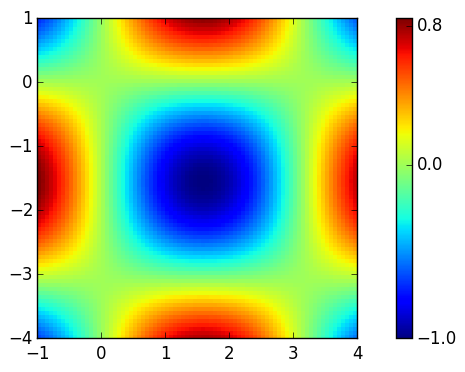
\includegraphics[width=\textwidth]{heatmap_color.png}
\end{subfigure}%
\begin{subfigure}{.5\textwidth}
  \centering
  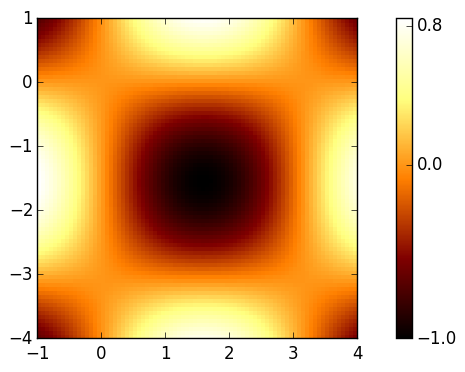
\includegraphics[width=\textwidth]{heatmap_hot.png}
\end{subfigure}
%\includegraphics[width=\textwidth]{heatmap.png}
\caption{Both of these pseudocolor plots depict the function $z = \sin(x)\sin(y)$ on the domain $[-1,4] \times [-4,1]$. 
The plot at left uses a rainbow gradient which is pretty to look at but whose choice of colors has no meaningful relationship to the data. 
The plot at right uses the colormap called \li{afmhot}, which has the important benefit that the lighter colors are naturally associated with higher values, while the darker colors are naturally associated with lower values.}
\label{fig:heatmap}
\end{figure}



You can also create a pseudocolor plot in matplotlib with the \li{plt.pcolormesh()} command.


One situation where heatmaps are very useful is when data is naturally associated to a geographic location.  When a heatmap is plotted on a map it is often called a \emph{cloropleth}.

TODO example of a cloropleth---maybe percentage income donated to charity by county? (makes Utah look good).

As in the case of a histogram, if the data is relatively coarse then the way the data is divided up can have an effect on the overall picture of the heatmap.

TODO make an example where things are binned in two different ways  and give a different-looking result.

\begin{problem}
TODO problem where data looks different when binned differently.  Have them make different choices and compare the results.
\end{problem}



Finally, three-dimensional data can also be plotted as a surface in 3-space, but it is often difficult to find a view where none of the important features of the data are obscured.
A heatmap can help avoid this problem and is often easier for the viewer to decode.

TODO give example of how the surface can obscure your view and how the contour or heatmap gives a clearer picture.


\section*{Exploring data with visualizations}
When you visualize data you may notice trends that are not apparent from the numbers. 
The following problem is a famous example of this phenomenon.

\begin{problem}\label{prob:anscombe}
The data sets I-IV in Table \ref{table:anscombe} are known as Anscombe's quartet. 
Each dat set has identical statistical properties. 
In each case,
\begin{itemize}
\item The mean of $x$ is 9 and the mean of $y$ is $7.5$.
\item The variance of $x$ is 11 and the variance of $y$ is 4.127.
\item The correlation between $x$ and $y$ is .816.
\item The linear regression line is $y=3+5x$.
\end{itemize}
Plot each data set. What do you notice?

\begin{table}[H]
\begin{tabular}{l l  |  l l  |  l l  |  l l }
I & & II & & III & & IV\\
x & y & x & y & x & y & x & y \\
\hline
10.0 & 8.04 & 10.0 & 9.14 & 10.0 & 7.46 & 8.0 & 6.58 \\
8.0 & 6.95 & 8.0 & 8.14 & 8.0 & 6.77 & 8.0 & 5.76 \\
13.0 & 7.58 & 13.0 & 8.74 & 13.0 & 12.74 & 8.0 & 7.71 \\
9.0 & 8.81 & 9.0 & 8.77 & 9.0 & 7.11 & 8.0 & 8.84 \\
11.0 & 8.33 & 11.0 & 9.26 & 11.0 & 7.81 & 8.0 & 8.47 \\
14.0 & 9.96 & 14.0 & 8.10 & 14.0 & 8.84 & 8.0 & 7.04 \\
6.0 & 7.24 & 6.0 & 6.13 & 6.0 & 6.08 & 8.0 & 5.25 \\
4.0 & 4.26 & 4.0 & 3.10 & 4.0 & 5.39 & 19.0 & 12.50 \\
12.0 & 10.84 & 12.0 & 9.13 & 12.0 & 8.15 & 8.0 & 5.56 \\
7.0 & 4.82 & 7.0 & 7.26 & 7.0 & 6.42 & 8.0 & 7.91 \\
5.0 & 5.68 & 5.0 & 4.74 & 5.0 & 5.73 & 8.0 & 6.89 \\
\end{tabular}
\caption{These four sets of data are known as Anscombe's quartet.}
\label{table:anscombe}
\end{table}
\end{problem}

As Problem \ref{prob:anscombe} demonstrates, a picture can quickly reveal properties of the data that are difficult to see in a list of numbers.

\subsection*{The Iterative Process of Exploratory Visualization} 

Understanding a data set through visualization is often an iterative process. We start with an initial visualization---usually a broad overview.  Examining the result leads to observations that provoke questions.  We then filter or transform the data and adjust the visualization based on those questions and observations, and then repeat the process until we converge on a useful result.

Some of the questions that you should be asking in this iterative process include:
\begin{enumerate}
\item Are the data correct and reliable? 
\item Are there any clear patterns, trends, or irregularities?
\item Would a different type of visualization give more information?
\item Is something unusual or interesting going on outside my view?
\item Would filtering the data to look at a particular subset give a more informative picture?
\item Would a transformation of the data give a more informative picture?
\end{enumerate}

\subsubsection*{Data integrity}

Visualization is a powerful way to identify problems with your data set.  Ask yourself, whether the results look like what you expect.  Are they the right magnitude? Are there missing values? 

TODO examples of visualizations that reveal these types of problems.

\subsubsection*{Trends, patterns, and irregularities}


Some patterns you may look for:
\begin{enumerate}
\item Are there trends in time (up, down, flat, cyclical)?
\item Does the data look random, cyclical, or patterned?
\item Are there clear correlations between the $x$- and $y$- values? 
\item Is the trend linear or curved?
\item Do lines intersect, or are they parallel?
\item Are the data symmetric or skewed?
\item What is the variance (wide vs narrow)?
\item Are there clusters and gaps?
\item Are the data dense or sparse?
\end{enumerate}

\subsubsection*{Using different types of visualization}

TODO examples

\begin{problem}
TODO problem: given one visualization, choose another type of vis and plot the data again with the new choice.  What are the relative merits of each?
\end{problem}


\subsubsection*{Changing the view}

By choosing to plot only a portion of your data, you may be able to focus your attention on the most relevant data.  On the other hand, you may also miss some interesting behavior in the data you didn't graph.

Another issue to consider is scale. If a number changes from 50,000 to 55,000 over some period, that  increase can appear small or large, depending on where we start the $y$-axis and how long we stretch out the $x$-axis (see Figure \ref{fig:dog_plots}).

You can modify the scale of an existing plot using \li{plt.yscale()} or \li{plt.xscale()}.

TODO more examples of zoom in or zoom out or different reference frame.

\begin{problem}
TODO problem changing the scale 
\end{problem}



\subsubsection*{Filtering the data}

Sometimes important information about a subset of the data can be obscured by considering the whole data set.  

TODO example where scatterplot of all people looks random, but separating by something like education level shows clear trends for one level. 


\subsubsection*{Transforming the data}

Often a transformation of the data can reveal useful information that was previously hidden.

For example, data that grows very rapidly or that is tightly clustered may be better visualized by plotting the logarithm of the data, instead of the original data, A log-lin plot (also called a log plot) is constructed by by taking the logarithm of only the $y$-values of your data set. 

This is easily done in matplotlib with the command \li{plt.semilogy(x,y)}.  The syntax is the same as \li{plt.plot}.

TODO example of basic line plot of $x^{14}$ versus $x^{13}$---looks identical inititally, but a log-lin plot shows they are very different.



Similarly, if the data grows very slowly, you may find that a lin-log plot (given by by taking the logarithm of only the $x$-values) gives a more useful view.
This is easily done in matplotlib with the command \li{plt.semilogy(x,y)}


TODO example of basic line plot of $x^{1/14}$ versus $x^{1/13}$---looks identical inititally, but a lin-log plot shows they are very different.


Transformations can also be useful for histograms.
As an example, let us look at the cost of health care claims. 
Our data set is bogus but created to closely resemble real-life data. 
An initial plotting of the data produces the histogram on the left in Figure \ref{fig:healthcare}. 
From this picture, it is hard to see the nature of the data---the plot just looks like a single bar. 
We may think that all health care claims are cheap. 
However, when we take the logarithm of the claims prices, we get the histogram on the right in Figure \ref{fig:healthcare}. 
Graphed on this scale, the data has a bell-shaped distribution similar to a normal distribution. 
Moreover, we see that there are some very expensive claims being submitted, though they are few. 
\begin{figure}
\centering
\begin{subfigure}{.5\textwidth}
  \centering
  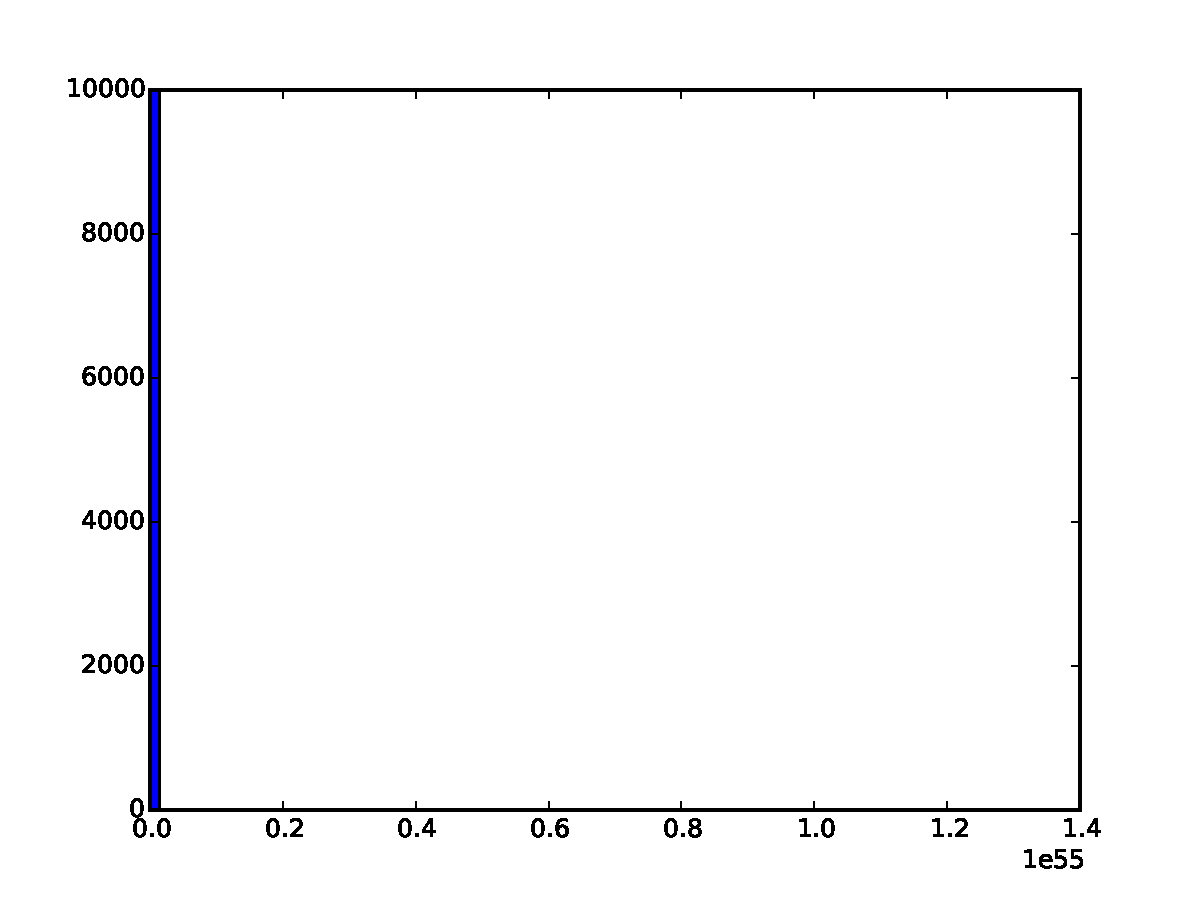
\includegraphics[width=\textwidth]{healthcare_linscale.pdf}
\end{subfigure}%
\begin{subfigure}{.5\textwidth}
  \centering
  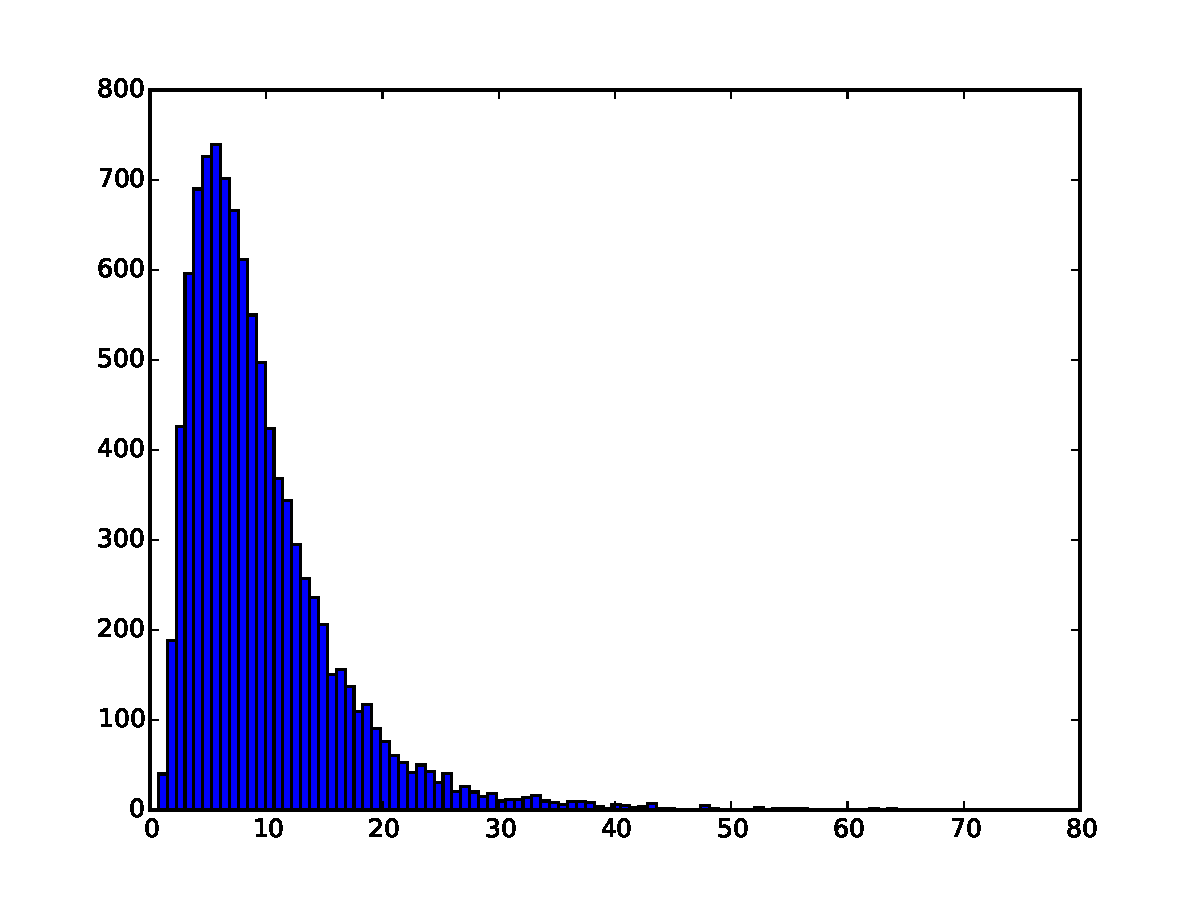
\includegraphics[width=\textwidth]{healthcare_logscale.pdf}
\end{subfigure}
\caption{The same data (meant to resemble the prices of health care claims) is plotted in both histograms above. 
The plot at left is a lin-lin scale, whereas the plot at right is a log-lin scale. 
In this case, changing scales revealed important information about the data.}
\label{fig:healthcare}
\end{figure}

As a general rule, log-lin plots are useful when the range of the $y$-values is orders of magnitude larger than the range of the $x$-values. 
Our health care data was an example of this. 
Similarly, lin-log plots are useful when the range of the $x$-values is much bigger than the range of the $y$-values. 
In any case, you can try applying a log scale to one or both of your axes as a way to explore your data.

Let us analyze the mathematics behind log plots. 
Suppose we have some data that roughly follows the line $y=cx^a$ where $c$ and $a$ are constants. 
Taking the logarithm of both sides yields
\[
\log(y) = a\log(x) + \log(c).
\]
If we set new variables $X = \log(x)$ and $Y = \log(y)$, then this equation becomes $Y = aX + \log(c)$, which is the equation of a straight line. 
So  on a log-log plot, polynomial-shaped data looks linear. 
Similarly, taking the log of $y = a^x$ yields
\[
\log(y) = \log(a)x,
\]
so exponential data looks linear on a log-lin plot. 
Finally, data of the form $y = a\log(x)+b$ will look linear on a lin-log plot. 
See Figure \ref{fig:log_plots}.

\begin{figure}
\centering
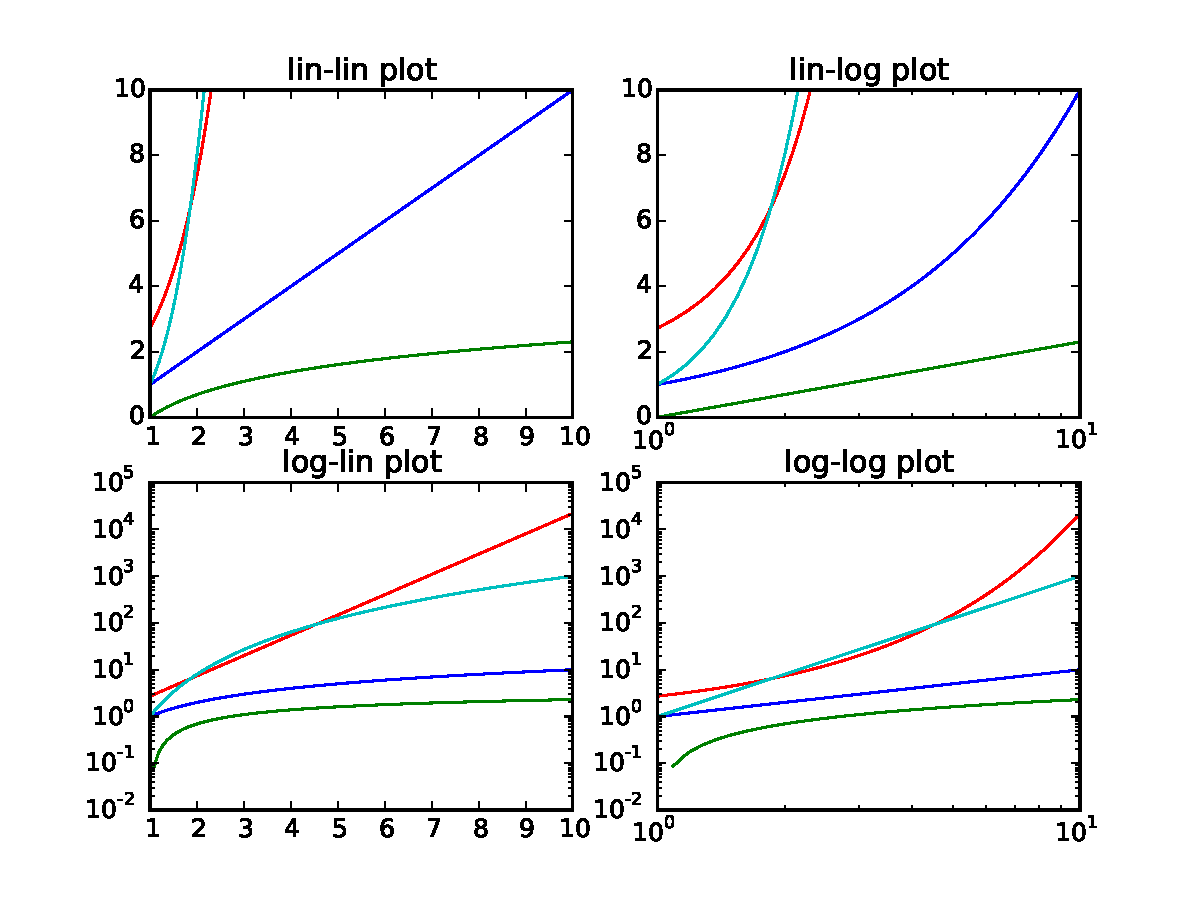
\includegraphics[width=\textwidth]{log_plots.pdf}
\caption{Here are some functions plotted on various logarithmic and linear scales. 
The dark blue line is $y=x$, the green line is $y=\log(x)$, the red line is $y=e^x$, and the light blue line is $y=x^3$. 
We have used different ranges on the $y$-axes to highlight appropriate parts of the graphs.}
\label{fig:log_plots}
\end{figure}

Be warned that many different functions can look linear on log plots. 
Thus, if you graph your data on a log-log plot and you see a line, you CANNOT conclude that your data must follow a polynomial. 
In general, you need more information.


\begin{problem}
Graph your data from Problem 1
TODO: fix this reference so that it is automatic, otherwise it will break if we rearrange sections.---end TODO
 in Lab \ref{lab:complexity} (Matrices and Complexity) on a (a) log-log scale, (b) log-lin scale, and (c) lin-log scale. 
Which plot makes the data easiest to understand?
\end{problem}


\begin{problem}

TODO: make a problem where they really explore some data, plot it in different ways, zoom in and out, and do a transformation.

\end{problem}



\section*{Communicating data with visualizations}

As the saying has it, ``a picture is worth a thousand words.'' 
Certainly, a data visualization is far more valuable than a thousand data points to a colleague who wants to understand the results of your analysis. 
Data visualizations are critical for communication in both business and research.

\subsection*{Choosing the right visualization}
At this point, you have already used visualization to explore your data and draw conclusions, and you are ready to tell your results to someone else. 
The first step in creating a graphic to do this is to choose the right type of visualization. 
As we saw in the section ``Types of Visualizations,'' there are many possibilities, each with different strengths. 
You should carefully consider which one best suits your data set and communication needs.  Your goal should always be communicating as clearly, effectively, and accurately as possible.  

\subsubsection*{Visualizations to avoid}
There are also several popular types of visualizations that you should generally \textbf{not} use.  These may look pretty, but they tend to obscure information or are easily confused, because of natural difficulties humans have interpreting them.

For example, people have much more difficulty judging changes and variation in area than they do in length.  
As a result, charts that depend on distinguishing variation in area will be less effective.  One of the most common charts that has this problem is the pie chart. 

TODO include examples showing how hard it is to distinguish size of wedges.

TODO convert the pie data to a good bar chart and show see how much better it is.

As bad as the pie chart may be, there is a way to make things worse---make the chart three-dimensional.  It seems to be very popular for people to convert a visualization that is naturally 2 or 1 dimensional into one that is artificially three dimensional, but this inevitably makes things more confusing.  For example, we already have difficulty distinguishing the variation in area in a pie chart, and when we add a third dimension, it becomes even harder.


TODO give example of A 3-d pie chart with the same data rotated to different sides and show how the slice look very different from different angles.


Other visualization types that tend to be confusing and ineffective include the stacked bar and the radar graph.  The radar graph is just generally confusing.  While problem with stacking bars is that the second bar is not based at zero, so it becomes difficult to compare the different parts.

TODO give an example of a stacked bar chart.  and then swap the data so the other set is on top and see that the reader has a totally different takeaway depending on how it is laid out.


In these examples differences in design give completely different impressions of the data, so the reality of the data is obscured rather than illuminated by the design.  As the famous visualization guru, Edward Tufte, says, ``Show data variation, not design variation.''  Pie charts and stacked bar charts show design variation more than data variation.


\subsection*{Simplify}

\noindent\emph{A sentence should contain no unnecessary words, a paragraph no unnecessary sentences for the same reason that a drawing should contain no unnecessary lines and a machine no unnecessary parts.} \small{---Strunk and White}


Once you have chosen the visualization best suited to your data, you should design the details so that all elements contribute to the communication of data. 

Edward Tufte offers two principles for simplifying graphics: (1) erase ink that does not communicate data, and (2) erase ink that communicates data redundantly.  (\cite{tufte2001} pp.96-100). According to these principles, decorative backgrounds, fancy lettering, and cute graphics in the corner of you plots should all be deleted.

Other opportunities for simplification are harder to notice and implement. As an example, let us examine the plot on the right of Figure \ref{fig:healthcare}. 
This plot was created with the following code.

\begin{lstlisting}
import numpy as np
import scipy as sp
from matplotlib import pyplot as plt

m = 2.07
s = 0.63
num_samples = 10000
samples = []

for i in xrange(num_samples):
    samples.append(sp.random.lognormal(m, s)) 

sp_samples = sp.array(samples)

# Plot the histogram
plt.hist(sp_samples, 100)
\end{lstlisting}

For purposes of this example, the only important part of the above code is the line \li{plt.hist(sp_samples, 100)} that plots the histogram. 
What ink in this plot can we erase because it communicates no data?

First, let's get rid of the vertical black lines that separate the bars of the histograph and the black outline. These are meaningless for our application and only distract. 
We can do this by modifying our call to \li{plt.hist()} as follows.

\begin{lstlisting}
plt.hist(sp_samples, 100, edgecolor='none')
\end{lstlisting}

Next, let us turn off the top and right lines that box in the graph. 
To do this, we need to access the ``axis'' object associated with the figure. 
We can access the ``axis'' object with the command \li{plt.gca()} (get current axis).

\begin{lstlisting}
# Get current axis instance
axis = plt.gca()

# Hide top and right spines
axis.spines['right'].set_visible(False)
axis.spines['top'].set_visible(False)
\end{lstlisting}

These commands only turn off the sides of the box, not the tick marks. 
To turn off the tick marks we run the following commands. 

\begin{lstlisting}
# Only show bottom and left tick marks
axis.yaxis.set_ticks_position('left')
axis.xaxis.set_ticks_position('bottom')
\end{lstlisting}

Finally, we do not need so many tick marks on the $x$- and $y$-axes. 
We adjust those along with specifying the range on each axis.

\begin{lstlisting}
# Fix x and y ranges
plt.xlim(0,70)
plt.ylim(0, 800)

# Use fewer axis ticks
plt.xticks(np.arange(0, 71, 35))
plt.yticks(np.arange(0, 801, 200))
\end{lstlisting}

The final graph is shown in Figure \ref{fig:simplify}. 
Note how much cleaner this looks than the original.

\begin{figure}
\centering
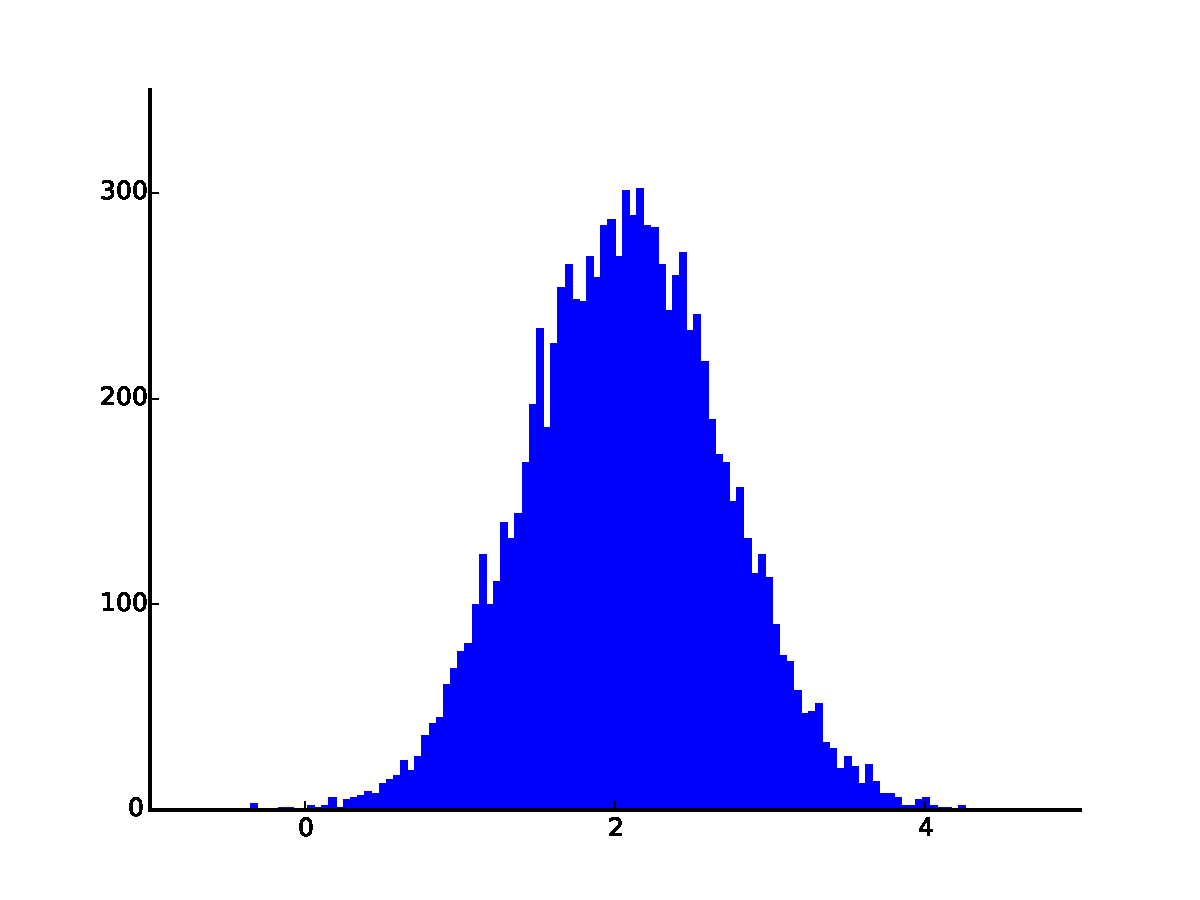
\includegraphics[width=\textwidth]{simplify.pdf}
\caption{A simplified version of the histogram in Figure \ref{fig:healthcare}.}
\label{fig:simplify}
\end{figure}


%TODO: Rewrite this problem to use a specific image with a specific context
\begin{problem}
Choose a graph you previously created that you think could use simplification. 
Apply at least 3 of the following to simplify your plot:
\begin{enumerate}
\item Turn off some of the spines.
\item Fix the x or y range to better fit your data.
\item Change the number of x or y ticks.
\item Choose a better color scheme.
\end{enumerate}
Simplify your image in any other ways you can think of.
\end{problem}

\subsection*{Small Multiples}

Often we have too much information to display cleanly in one chart.  One indicator of this is if the reader must often look back and forth between a legend and the chart to decode the images.  A very useful way to deal with this problem is the method of \emph{small multiples}, an idea made famous by Edward Tufte.

The idea is to separate the data into many small graphics, placed near each other in a way that allows us to easily compare them.

For example, one might wish to compare the first six Chebyshev polynomials.  It would be natural to plot them together on the same graph, as in Figure TODO.  But this graph is too cluttered and one must constantly refer back to the legend to identify which colored line is which.

TODO insert cluttered chebyshev graph.

The small multiple approach is to plot each polynomial on its own set of axes, adjacent to each other and aligned in such a way that you can easily compare the different plots. 

TODO insert small multiples of chebyshev

Note how even with 9 plots instead of 6, it is much easier to identify the different polynomials and to compare them.


TODO include the code for the small multiples.

The main tool you need to make small multiples is the command \li{ax = plt.subplot()}.  This allows you to set up multiple plots, and access them one at a time.


\begin{problem}

TODO make a problem where they plot small multiples of something and compare to the cluttered verison on top of each other.

\end{problem}

\subsection*{Tell the truth}

Just as graphics can tell your reader about your data, they can also give your viewer false impressions. 
You should never use data visualizations to mislead your reader. 
There are many ways pictures can be used to lie, and some of them can be unintentional.

\subsubsection*{2- and 3-d effects}
For example, if we see differences in flat shapes by area, not width or height. 
Suppose you are creating a pictogram to demonstrate the recent increase in housing prices, which have doubled in the last $n$ years. 
So, you draw two houses, one whose sides are 1cm and one whose sides are 2cm. 
The area of the second house is now $2^2=4$ times as big as the area of the first. And your reader will likely interpret the picture as a four-fold increase rather than just double. 
Hence, you should make two-dimensional pictures proportional in \emph{area} to the numbers they represent.

Even worse, volume is cubed rather than squared, so if a picture is intended to look like a three-dimensional object, doubling the side lengths will give the impression of an eight-fold increase.

TODO add figures with 2- and 3-d houses doubling in side length.

Three-dimensional special effects also tend to be misleading.  As mentioned above, a 3-D pie chart, for example, can be used to distort the sizes of its slices. 
Similarly, a 3-D histogram can use perspective to distort the relative differences between bars.

\subsubsection*{Base, Scale, and Labels}  

As mentioned above, bar charts should be based at 0 and all charts should be scaled in the way the most clearly conveys the most important and relevant information.  When there is a possibility of confusion, axes and key data values should be labeled for clarity.


\begin{figure}
\centering
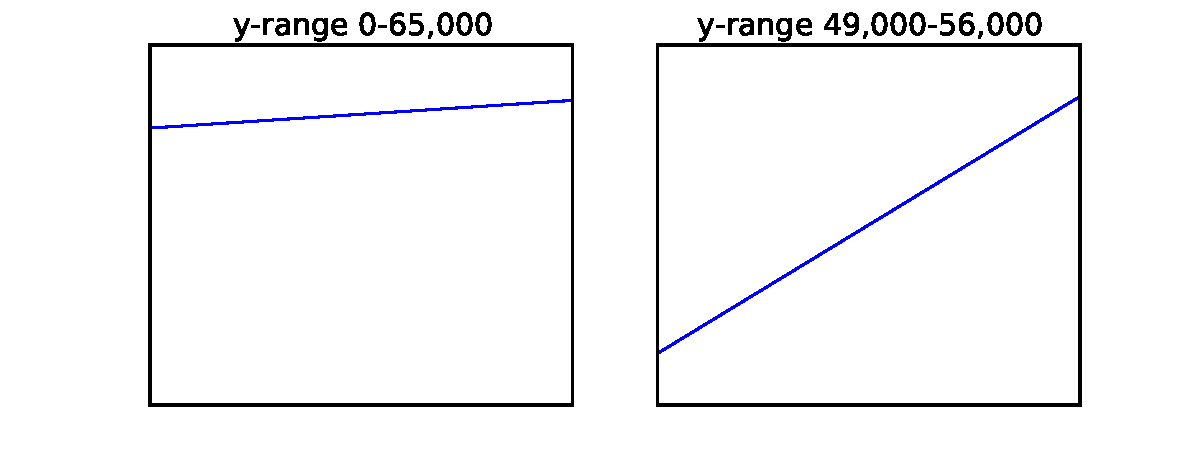
\includegraphics[width=\textwidth]{dog_plots.pdf}
\caption{The graph of some data can look very different depending on the scale. 
Here are two graphs of the ``same'' line over the same range (1 to 4). 
The only difference is the $y$-range. Notice easy it is to manipulate the y-scale to imply either a large or small increase in $y$. 
These figures are especially misleading when we leave the range markers off of the $y$-axes.}
\label{fig:dog_plots}
\end{figure}

As in any form of communication, integrity is important in data visualization. 
You will win more respect for yourself and those you represent if you avoid misleading diagrams.


\subsection*{Additional Resources}

There are many software packages that facilitate the visual exploration of data. 
One Python library is Glue (see \cite{glue}).

Some packages for making nicer looking plots include \li{Seaborn} and \li{prettyplotlib}.  TODO get refs

For more about visualization of data, we highly recommend the following books:

TODO get full refs for the follwoing

\begin{itemize}
\item \emph{How to lie with statistics}
\item \emph{Envisioning Information} by Edward Tufte
\item \emph{The visual display of quantitative information} by Edward Tufte (2nd edition)
\item \emph{Now you see it} by Stephen Few
\end{itemize}



\printbibliography